\documentclass[12pt]{article}

\usepackage{answers}
\usepackage{float}
\usepackage{setspace}
\usepackage{graphicx}
\usepackage{enumitem}
\usepackage{multicol}
\usepackage{mathrsfs}
\usepackage{listings}
\usepackage[margin=1in]{geometry} 
\usepackage{amsmath,amsthm,amssymb}
 
\usepackage[margin=0cm]{caption}
 
\newcommand{\N}{\mathbb{N}}
\newcommand{\Z}{\mathbb{Z}}
\newcommand{\C}{\mathbb{C}}
\newcommand{\R}{\mathbb{R}}

\DeclareMathOperator{\sech}{sech}
\DeclareMathOperator{\csch}{csch}
 
\newenvironment{theorem}[2][Theorem]{\begin{trivlist}
\item[\hskip \labelsep {\bfseries #1}\hskip \labelsep {\bfseries #2.}]}{\end{trivlist}}
\newenvironment{definition}[2][Definition]{\begin{trivlist}
\item[\hskip \labelsep {\bfseries #1}\hskip \labelsep {\bfseries #2.}]}{\end{trivlist}}
\newenvironment{proposition}[2][Proposition]{\begin{trivlist}
\item[\hskip \labelsep {\bfseries #1}\hskip \labelsep {\bfseries #2.}]}{\end{trivlist}}
\newenvironment{lemma}[2][Lemma]{\begin{trivlist}
\item[\hskip \labelsep {\bfseries #1}\hskip \labelsep {\bfseries #2.}]}{\end{trivlist}}
\newenvironment{exercise}[2][Exercise]{\begin{trivlist}
\item[\hskip \labelsep {\bfseries #1}\hskip \labelsep {\bfseries #2.}]}{\end{trivlist}}
\newenvironment{solution}[2][Solution]{\begin{trivlist}
\item[\hskip \labelsep {\bfseries #1}]}{\end{trivlist}}
\newenvironment{problem}[2][Problem]{\begin{trivlist}
\item[\hskip \labelsep {\bfseries #1}\hskip \labelsep {\bfseries #2.}]}{\end{trivlist}}
\newenvironment{question}[2][Question]{\begin{trivlist}
\item[\hskip \labelsep {\bfseries #1}\hskip \labelsep {\bfseries #2.}]}{\end{trivlist}}
\newenvironment{corollary}[2][Corollary]{\begin{trivlist}
\item[\hskip \labelsep {\bfseries #1}\hskip \labelsep {\bfseries #2.}]}{\end{trivlist}}
 
\begin{document}
 
% --------------------------------------------------------------
%                         Start here
% --------------------------------------------------------------
 
\title{Homework 1}%replace with the appropriate homework number
\author{Christian Steinmetz\\ %replace with your name
MATH 8090-Spring 2018} %if necessary, replace with your course title
 
\maketitle
\begin{problem}{7}
Consider fitting a model to the log of the Australian wine sales. Fit a model allowing for a term for each month. Fit the model with linear trend and monthly variables, plot the data and overlay the estimated values from the fitted model. Does it appear to provide a better fit than the sin/cos model from ppt? Use the Box test to test if there is significant autocorrelation in the residuals.
\end{problem}

\begin{solution}{}
The new model is shown in Figure \ref{fig:monthly_model} and appears to fit the data better than the sine and cosine model from class. The results from the box text are shown below. 

\begin{lstlisting}
Box-Ljung test
data:  lsfit$res
X-squared = 71.29, df = 15, p-value = 2.629e-09
\end{lstlisting}

\noindent
A $p-value << 0.05$ indicates that there is still autocorrelation present in the fitted model.
\vspace*{-1cm}
\begin{figure}[H]
    \centering
    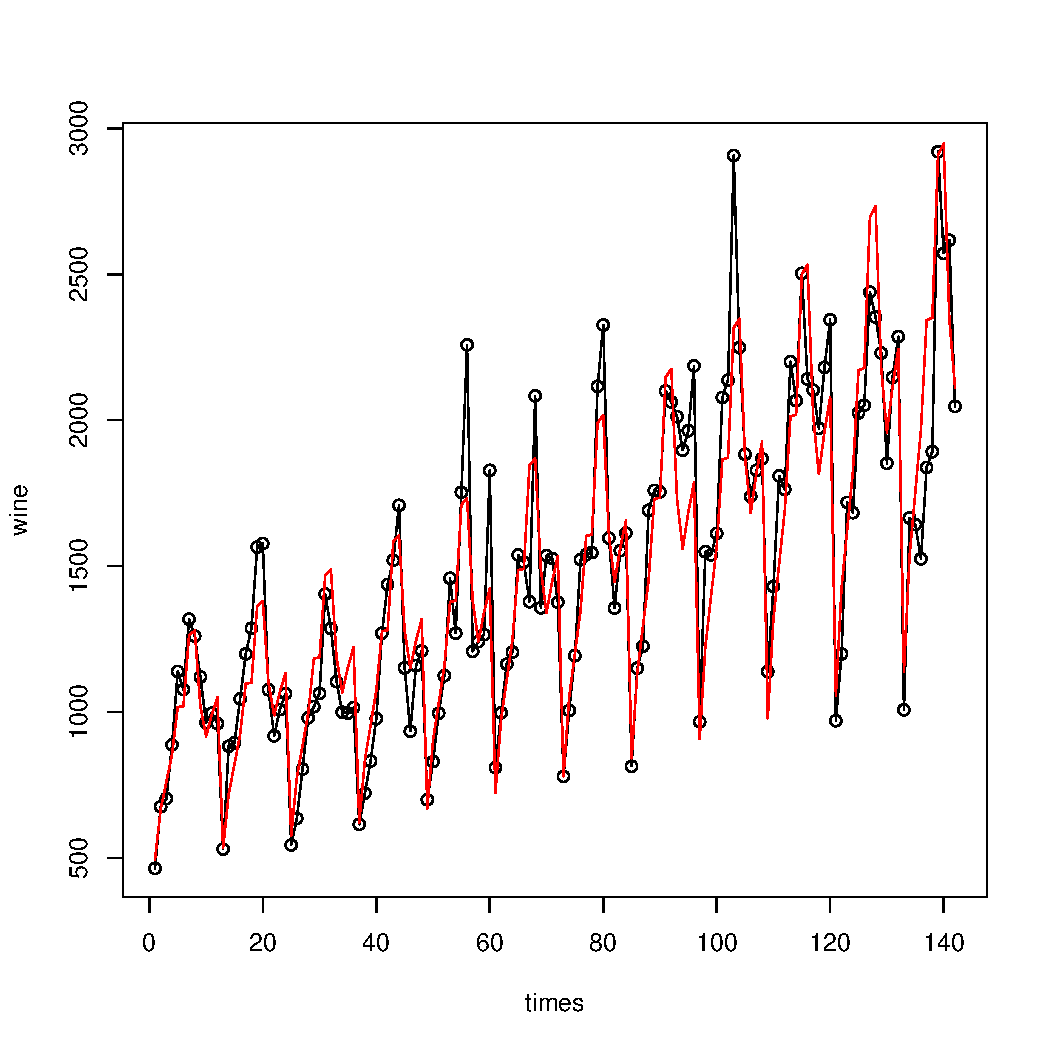
\includegraphics[width=0.6\textwidth]{figs/problem_7/monthly_model.pdf}
    \caption{Model with linear trend and monthly variables.}
    \label{fig:monthly_model}
\end{figure}

\end{solution}
\pagebreak

\begin{problem}{8}
Consider the global temperature deviations. Allow for a quadratic trend with AR(1) errors. You can mimic the R code for the lake Huron data. \begin{enumerate}[label=(\alph*)]
    \item Are the coefficients for both linear and quadratic terms statistically significant?  If not, drop that term and refit with just a linear trend.
    \item Make a 95\% confidence interval for the rate of change and interpret the limits of this interval in terms of temperature increase per century.  
\end{enumerate}
\end{problem}

\begin{solution}{}
$ $
\begin{enumerate}[label=(\alph*)]
    \item The quadratic model was fitted first and is shown in Figure \ref{fig:temp_ar1_quad}. The results from the ARIMA model are shown below.
    \begin{lstlisting}
Coefficients:
         ar1  intercept   times   tsqr
      0.4180    -0.5108  0.0110  -1e-04
s.e.  0.1752     0.0615  0.0028   2e-04

sigma^2 estimated as 0.01477: 
log likelihood = 74.28, aic = -138.56
    \end{lstlisting} 
    Since $|{\frac{-1e-04}{\phantom{-}2e-04}}| = \frac{1}{2} < 1.96$, the quadratic term is not significant. Therefore we refit the with a linear model, dropping the quadratic term. The output of this model is shown in Figure \ref{fig:temp_ar1_lin}, and we observe that the fit is similar. The output of the new ARIMA model is shown below. Notice that the times values are clearly significant. 
    \begin{lstlisting}
Coefficients:
         ar1  intercept   times
      0.4877    -0.4126  0.0056
s.e.  0.0836     0.0459  0.0007

sigma^2 estimated as 0.01534: 
log likelihood = 72.18, aic = -136.35
    \end{lstlisting}
    \item Based on our fitted model, we estimate with 95\% confidence that the average rate of change of the global temperature is increasing by at least $(0.0056-(1.645*0.0007)) = 0.0044485$ degrees per year or $0.44485$ degrees per century. 
\end{enumerate}

\vspace*{-4cm}
\begin{figure}
    \centering
    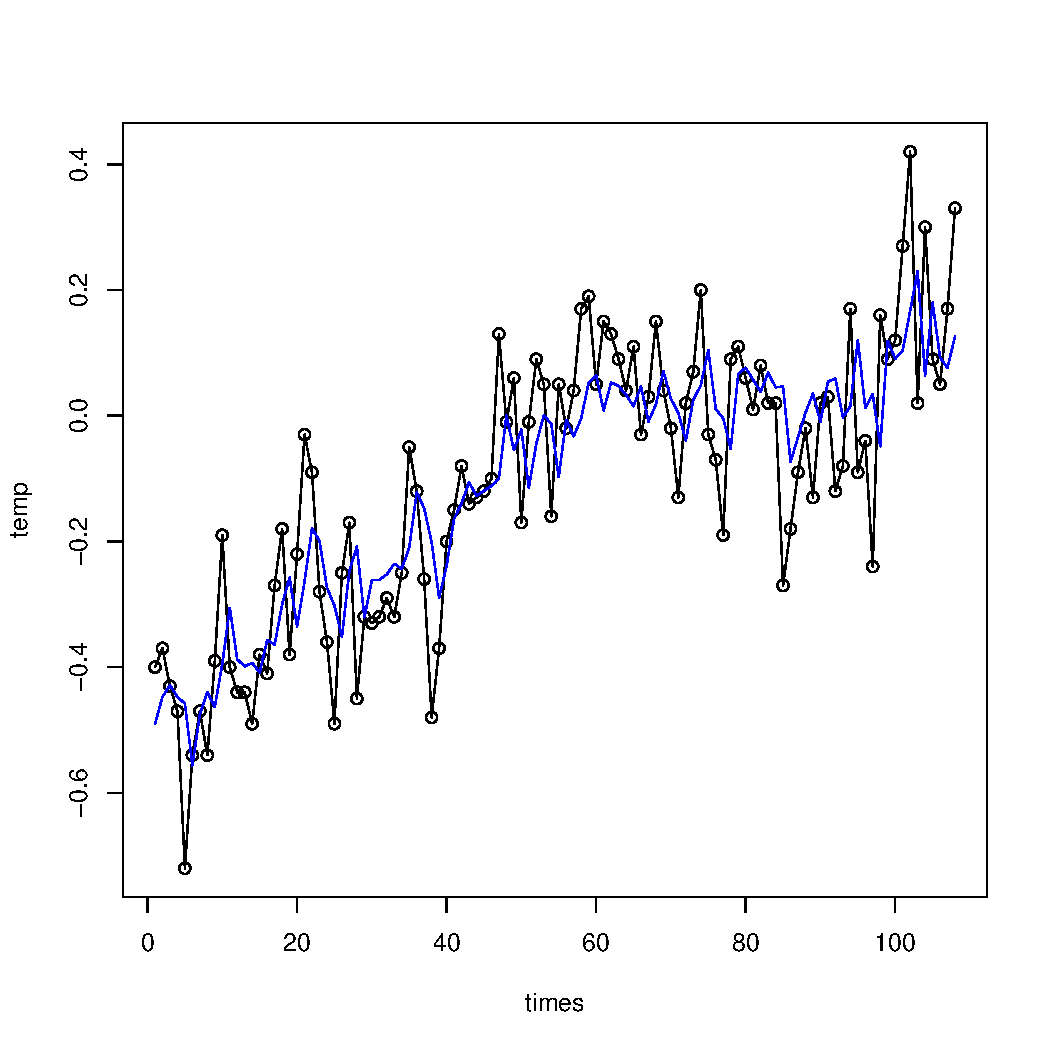
\includegraphics[width=0.6\textwidth]{figs/problem_8/temp_ar1_quad.pdf}
    \vspace*{-0.5cm}
    \caption{Quadratic model with AR(1) errors.}
    \label{fig:temp_ar1_quad}
\end{figure}
\vspace*{-4cm}
\begin{figure}
    \centering
    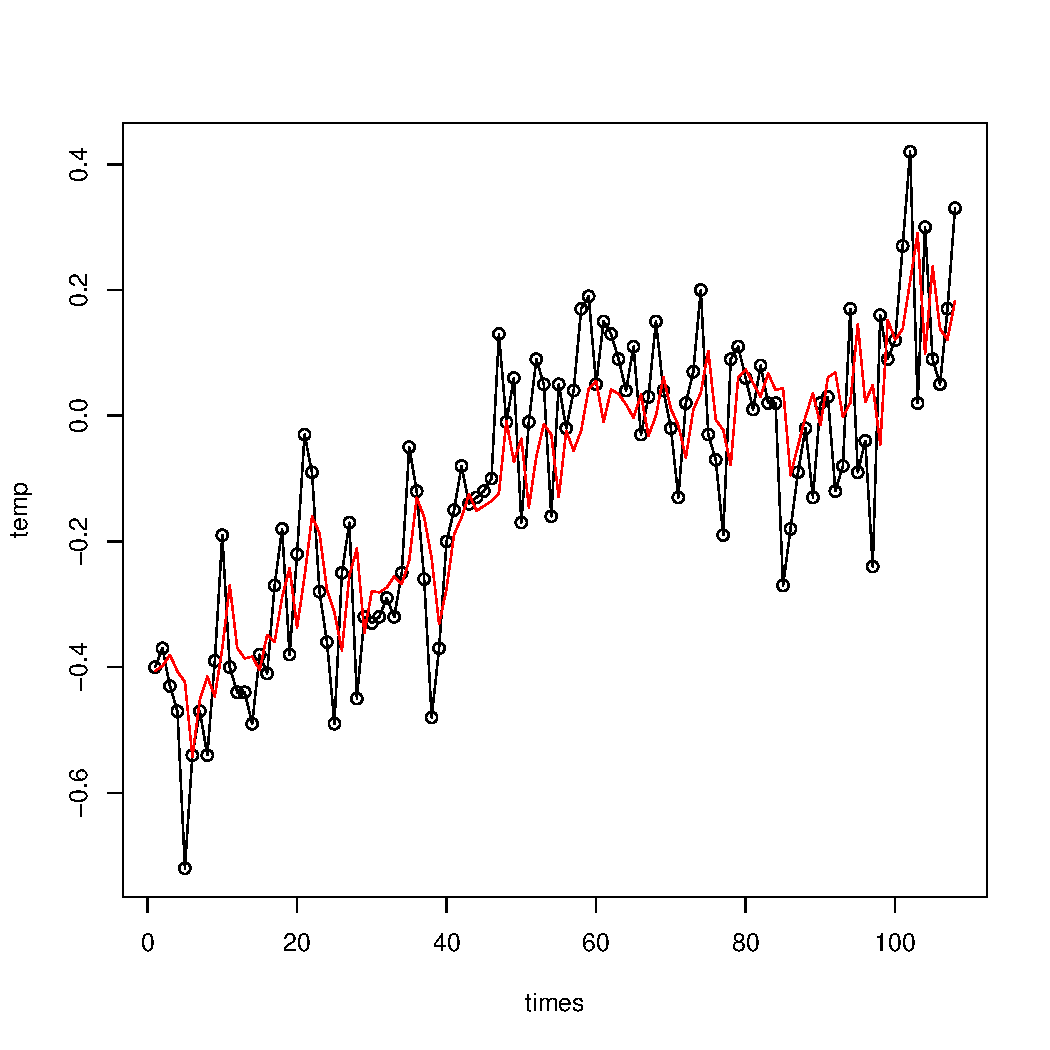
\includegraphics[width=0.6\textwidth]{figs/problem_8/temp_ar1_lin.pdf}
    \vspace*{-0.5cm}
    \caption{Linear model with AR(1) errors.}
    \label{fig:temp_ar1_lin}
\end{figure}


\end{solution}
\pagebreak

\begin{problem}{9}
Use R to
\begin{enumerate}[label=(\alph*)]
    \item fit a cubic trend to the lake data: $X_t=\beta_0+\beta_1t+\beta_2t^2+\beta_3t^3+Y_t$.
    \item plot the lake data with estimated cubic trend overlay.
\end{enumerate}
Find residuals from the estimated trend and plot the sample ACF. Use the Ljung- Box test to check for statistically significant autocorrelation. 
\end{problem}

\begin{solution}{}
$ $
\begin{enumerate}[label=(\alph*)]
    \item The fitted trend is shown from the output below.
    \begin{lstlisting}
              Estimate  Std. Error t value Pr(>|t|)
(Intercept)  1.131e+01  4.327e-01  26.129   <2e-16 ***
Xtimes      -8.972e-02  3.766e-02  -2.383   0.0192 *
X            6.415e-04  8.814e-04   0.728   0.4686
X            2.288e-07  5.854e-06   0.039   0.9689
    \end{lstlisting}
    \item The cubic trend is shown in Figure \ref{fig:cubic_fit}.
\end{enumerate}

\begin{figure}[h]
    \vspace*{-1cm}
    \centering
    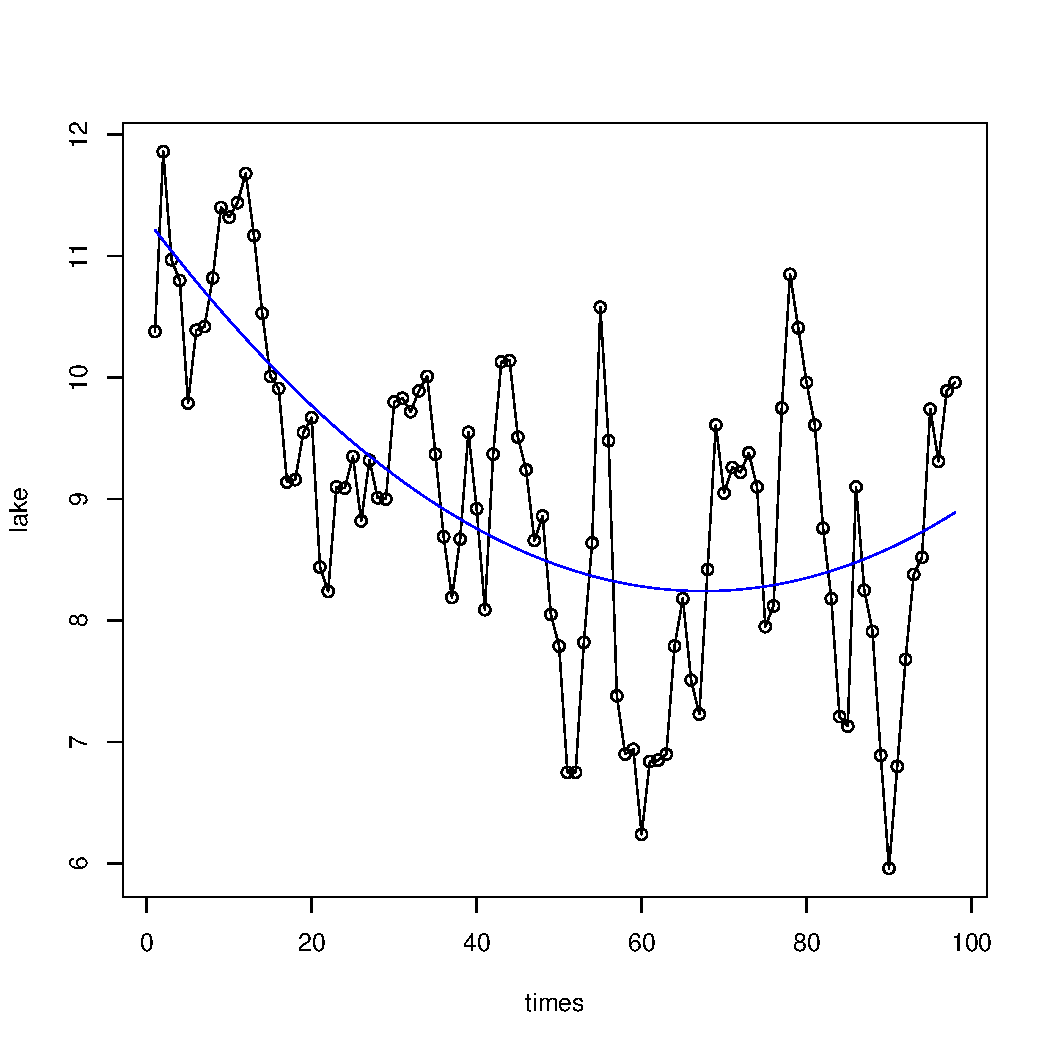
\includegraphics[width=0.8\textwidth]{figs/problem_9/cubic_fit.pdf}
    \vspace*{-0.5cm}
    \caption{Cubic model for the Lake Huron data.}
    \label{fig:cubic_fit}
\end{figure}

\begin{figure}[h]
    \centering
    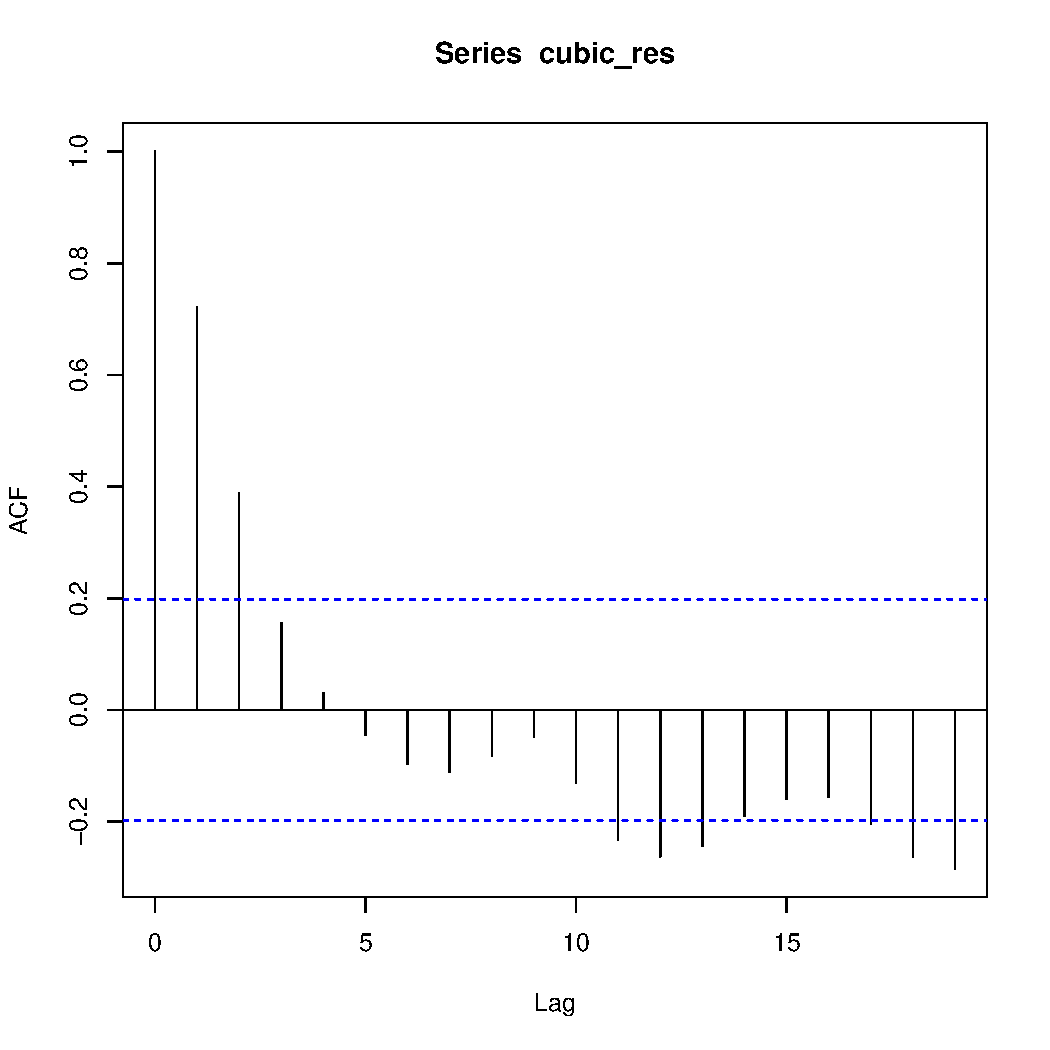
\includegraphics[width=0.8\textwidth]{figs/problem_9/cubic_fit_ACF.pdf}
    \vspace*{-0.5cm}
    \caption{Cubic model for the Lake Huron data.}
    \label{fig:cubic_fit_ACF}
\end{figure}
\newpage
\noindent
A box plot of the residuals from the model is shown in Figure \ref{fig:cubic_fit_ACF}. Significant autocorrelation is observed at multiple lags after lag 0. The Ljung Box Test confirms this. Its output is shown below. 

\begin{lstlisting}
Box-Ljung test
data:  cubic_res
X-squared = 103.9, df = 15, p-value = 2.331e-15
\end{lstlisting}

\noindent
A $p-value << 0.05$ indicates that there is still autocorrelation present in the fitted model.

\end{solution}
\pagebreak

\begin{problem}{10}
Rather than estimate first order trend and seasonal components, we can use differencing. In R we can difference using diff(data,lag,times) where lag determines the lag at which we difference (at the period for seasonal data) and times determines how many times (k to remove a kth order polynomial). 
\begin{enumerate}[label=(\alph*)]
    \item Difference the log of wines sales at lag=12. Plot the differenced data. Does there appear to be any remaining trend?  Test for autocorrelation in differences using Box-Ljung. Notice the differencing removes first order, but not second order effects!
    \item  Difference the baseball data at lag=1. Plot the differenced data and test for autocorrelation.    
\end{enumerate}
\end{problem}

\begin{solution}{}
$ $
\begin{enumerate}[label=(\alph*)]
    \item The differenced wine data is shown in Figure \ref{fig:wine_diff} and the result of the Ljung Box Test is shown below.
    \begin{lstlisting}
Box-Ljung test
data:  y_diff
X-squared = 63.636, df = 15, p-value = 5.917e-08
    \end{lstlisting}
    A $p-value << 0.05$ indicates that there is still autocorrelation present in the fitted model, even once we performed first order differencing on the data.
    \item The differenced wine data is shown in Figure \ref{fig:baseball_diff} and the result of the Ljung Box Test is shown below.
    \begin{lstlisting}
Box-Ljung test
data:  baseball_diff
X-squared = 13.502, df = 15, p-value = 0.5636
    \end{lstlisting}
    A $p-value > 0.05$ indicates there is likely no autocorrelation present in the fitted model once we performed first order differencing on the data.
\end{enumerate}

\begin{figure}
    \centering
    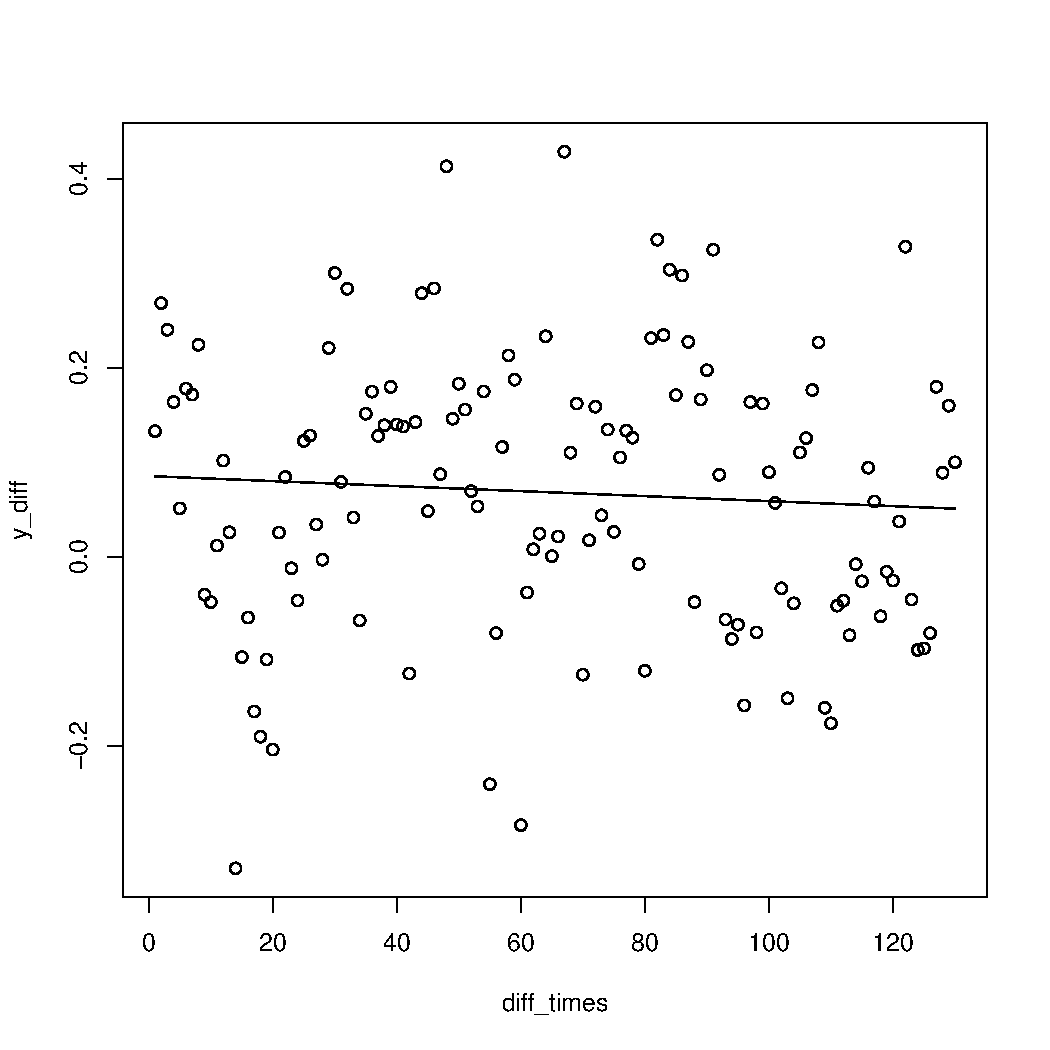
\includegraphics[width=0.8\textwidth]{figs/problem_10/wine_diff_lag12.pdf}
    \vspace*{-0.5cm}
    \caption{First order differncing on wine data with lag=12.}
    \label{fig:wine_diff}
\end{figure}

\begin{figure}
    \centering
    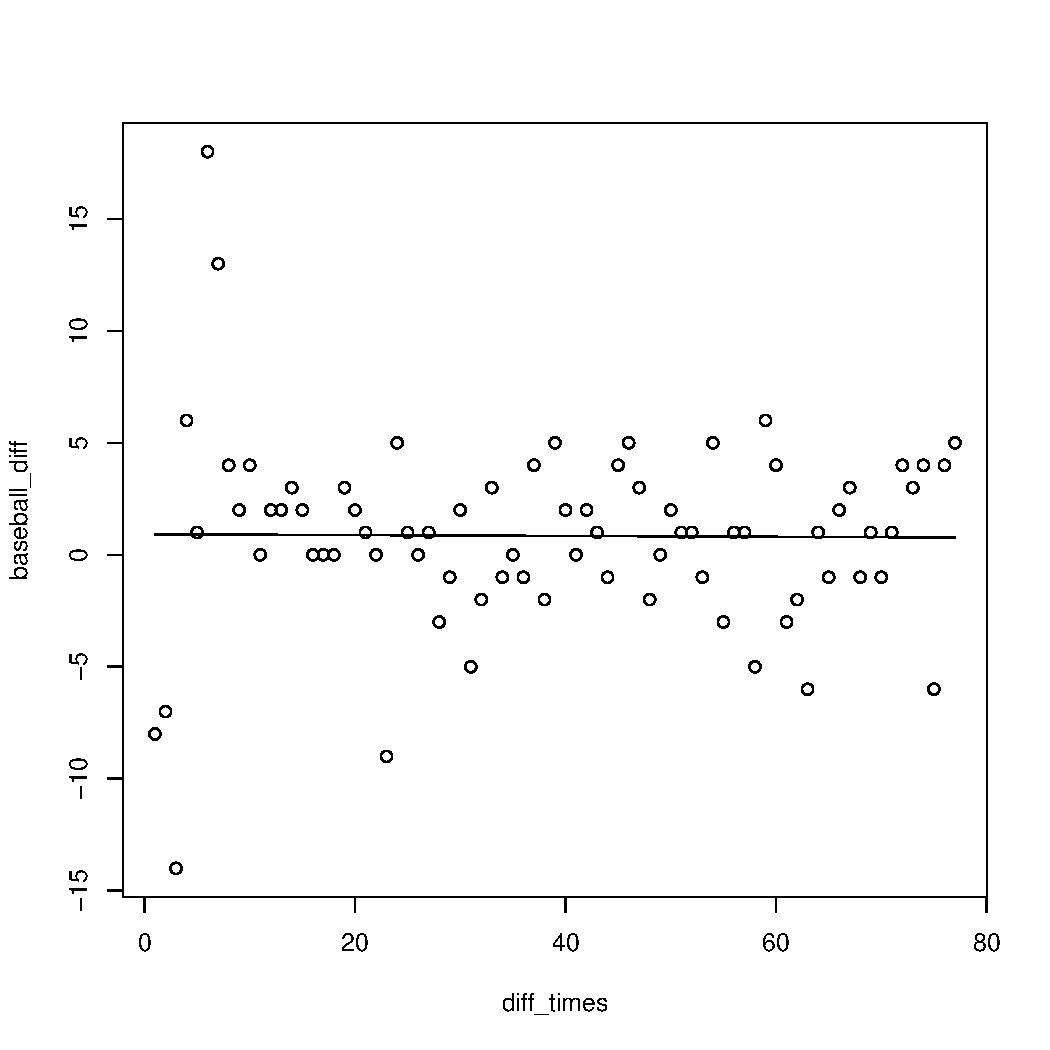
\includegraphics[width=0.8\textwidth]{figs/problem_10/baseball_diff_lag1.pdf}
    \vspace*{-0.5cm}
    \caption{First order differncing on baseball data with lag=1.}
    \label{fig:baseball_diff}
\end{figure}

\end{solution}

\end{document}
